\documentclass[12pt, titlepage]{article}

\usepackage{fullpage}
\usepackage[round]{natbib}
\usepackage{multirow}
\usepackage{booktabs}
\usepackage{tabularx}
\usepackage{graphicx}
\usepackage{float}
\usepackage{hyperref}
\usepackage[table]{xcolor} 
\hypersetup{
    colorlinks,
    citecolor=blue,
    filecolor=black,
    linkcolor=red,
    urlcolor=blue
}

%% Comments

\usepackage{color}

%\newif\ifcomments\commentstrue %displays comments
\newif\ifcomments\commentsfalse %so that comments do not display

\ifcomments
\newcommand{\authornote}[3]{\textcolor{#1}{[#3 ---#2]}}
\newcommand{\todo}[1]{\textcolor{red}{[TODO: #1]}}
\else
\newcommand{\authornote}[3]{}
\newcommand{\todo}[1]{}
\fi

\newcommand{\wss}[1]{\authornote{blue}{SS}{#1}} 
\newcommand{\plt}[1]{\authornote{magenta}{TPLT}{#1}} %For explanation of the template
\newcommand{\an}[1]{\authornote{cyan}{Author}{#1}}

%% Common Parts

\newcommand{\progname}{Mechatronics Engineering} % PUT YOUR PROGRAM NAME HERE
\newcommand{\authname}{Team 25, Preliminary
\\ Ahmed Nazir, nazira1
\\ Stephen Oh, ohs9
\\ Muhanad Sada, sadam
\\ Tioluwalayomi Babayeju, babayejt} % AUTHOR NAMES                  

\usepackage{hyperref}
    \hypersetup{colorlinks=true, linkcolor=blue, citecolor=blue, filecolor=blue,
                urlcolor=blue, unicode=false}
    \urlstyle{same}
                                


\newcounter{acnum}
\newcommand{\actheacnum}{AC\theacnum}
\newcommand{\acref}[1]{AC\ref{#1}}

\newcounter{ucnum}
\newcommand{\uctheucnum}{UC\theucnum}
\newcommand{\uref}[1]{UC\ref{#1}}

\newcounter{mnum}
\newcommand{\mthemnum}{M\themnum}
\newcommand{\mref}[1]{M\ref{#1}}

\begin{document}

\title{System Design for \progname{}} 
\author{\authname}
\date{\today}

\maketitle

\pagenumbering{roman}

\section{Revision History}

\begin{tabularx}{\textwidth}{p{3cm}p{2cm}X}
\toprule {\bf Date} & {\bf Version} & {\bf Notes}\\
\midrule
Date 1 & 1.0 & Notes\\
Date 2 & 1.1 & Notes\\
\bottomrule
\end{tabularx}

\newpage

\section{Reference Material}

This section records information for easy reference.

\subsection{Abbreviations and Acronyms}

\renewcommand{\arraystretch}{1.2}
\begin{tabular}{l l} 
  \toprule		
  \textbf{symbol} & \textbf{description}\\
  \midrule 
  \progname & Explanation of program name\\
  \wss{...} & \wss{...}\\
  \bottomrule
\end{tabular}\\

\newpage

\tableofcontents

\newpage

\listoftables

\listoffigures

\newpage

\pagenumbering{arabic}

\section{Introduction}

\wss{Include references to your other documentation}

\section{Purpose}

\wss{Purpose of your design documentation}

\wss{Point to your other design documents}

\section{Scope}

\wss{Include a figure that show the System Context (showing the boundary between
your system and the environment around it.)}

\section{Project Overview}

\subsection{Normal Behaviour}

\subsection{Undesired Event Handling}

\wss{How you will approach undesired events}

\subsection{Component Diagram}

\subsection{Connection Between Requirements and Design} \label{SecConnection}

\wss{The intention of this section is to document decisions that are made
  ``between'' the requirements and the design.  To satisfy some requirements,
  design decisions need to be made.  Rather than make these decisions implicit,
  they are explicitly recorded here.  For instance, if a program has security
  requirements, a specific design decision may be made to satisfy those
  requirements with a password.}

\section{System Variables}

\wss{Include this section for Mechatronics projects}

\subsection{Monitored Variables}
  \begin{tabular}{| p{0.23\textwidth} | p{0.10\textwidth}| p{0.10\textwidth}| p{0.46\textwidth}|}
    \hline
    \rowcolor[gray]{0.9}
    Monitored Variable & Type & Units & Description\\
    \hline
    m\_vibration & Analog& V& A signal monitoring the vibration resistance of the motor \\
    \hline
    m\_humidity & Analog & V & A signal monitoring the humidity of the motor’s environment \\
    \hline
    m\_temperature & Analog & V & A signal monitoring the temperature of the motor’s environment \\
    \hline
    m\_shock & Analog & V & A signal monitoring the shock resistance of the motor \\
    \hline
    m\_conv\_vibration & Digital & g  & Converted vibration values that are in useful units \\
    \hline
    m\_conv\_humidity & Digital & \% & Converted humidity values that are in useful units \\
    \hline
    m\_conv\_temperature & Digital & \textdegree C & Converted temperature values that are in useful units \\
    \hline
    m\_conv\_shock & Digital & g & Converted shock values that are in useful units \\
    \hline
    m\_data\_accepted & Digital & T/F & Determines if user has accepted the results and wants to send it to the database \\
    \hline
  \end{tabular}

\subsection{Controlled Variables}
  \begin{tabular}{| p{0.23\textwidth} | p{0.10\textwidth}| p{0.10\textwidth}| p{0.46\textwidth}|}
    \hline
    \rowcolor[gray]{0.9}
    Controlled Variable & Type & Units & Description\\
    \hline
    c\_green\_light& Digital& 1/0& Green LED light on testing device that indicates passed measurements \\
    \hline
    c\_red\_light& Digital & 1/0 & Red LED light on testing device that indicates failed measurements \\
    \hline
    c\_sent\_to\_database & Digital & T/F & Determines if results displayed on the application are sent to the database \\
    \hline
  \end{tabular}

\subsection{Constants Variables}
  \begin{tabular}{| p{0.23\textwidth} | p{0.10\textwidth}| p{0.10\textwidth}| p{0.46\textwidth}|}
    \hline
    \rowcolor[gray]{0.9}
    Constant & Units & Value & Description\\
    \hline
    k\_temperature\_range& \textdegree C& 5-40& Acceptable ambient temperature values for a Formula Electric motor \\
    \hline
    k\_humidity\_range& \% & 5-85 & Acceptable relative humidity values for a Formula electric motor \\
    \hline
    k\_max\_shock & g & 100 & Maximum shock resistance for a Formula Electric motor \\
    \hline
    k\_max\_vibration & g & 20 & Maximum vibration resistance for a Formula Electric motor \\
    \hline
  \end{tabular}

\section{User Interfaces}

\subsection{Desktop Application}
The user interface for the desktop application is designed through Qt designer, a software for designing and building GUIs through the Qt library. Qt designer generates UI files which can be converted to python scripts that build the static design and layout of the GUI. The desktop application is essentially multiple pages stacked on each other that change based on which buttons are clicked. The GUI is comprised of a left bar menu, top bar, and content pages being in the center, refer to figure 1 and 2 in the Appendix. Navigation through the application is done using the sidebar menu, where users can toggle the full menu and press on which page they want to go. The top bar will be used for extra functionality such as accessing user details, minimizing screen, etc. Users interact with the application using buttons to perform a variety of functions and form fields in which they can enter test/user information.

\wss{Design of user interface for software and hardware.  Attach an appendix if
needed. Drawings, Sketches, Figma}

\section{Design of Hardware}

\wss{Most relevant for mechatronics projects}
\wss{Show what will be acquired}
\wss{Show what will be built, with detail on fabrication and materials}
\wss{Include appendices as appropriate, possibly with sketches, drawings, CAD, etc}

\section{Design of Electrical Components}

\wss{Most relevant for mechatronics projects}
\wss{Show what will be acquired}
\wss{Show what will be built, with detail on fabrication and materials}
\wss{Include appendices as appropriate, possibly with sketches, drawings,
circuit diagrams, etc}

\section{Design of Communication Protocols}

\wss{If appropriate}

\section{Timeline}

\wss{Schedule of tasks and who is responsible}

% \bibliographystyle {plainnat}
% \bibliography{../../../refs/References}

\newpage{}

\appendix

\section{Interface}
\begin{figure}[h!]
  \begin{center}
  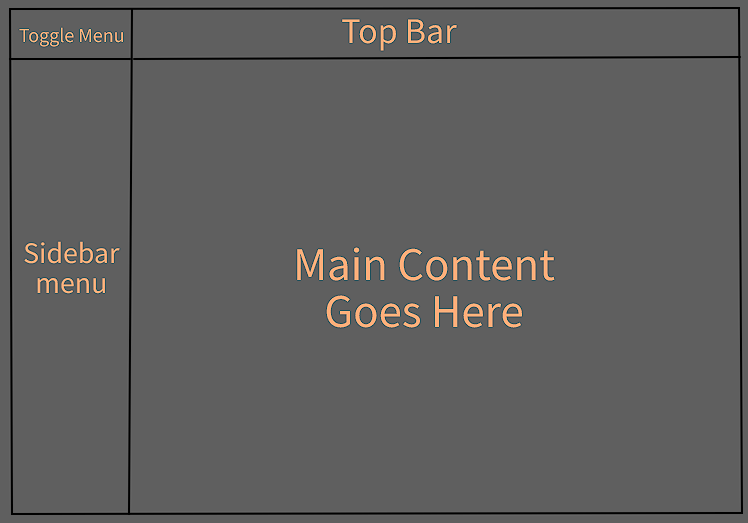
\includegraphics[width=0.9\textwidth]{GUI_sketch}
  \caption{Basic layout of GUI}
  \label{Fig_SystemContext} 
  \end{center}
  \end{figure}

\begin{figure}[hbt!]
  \begin{center}
  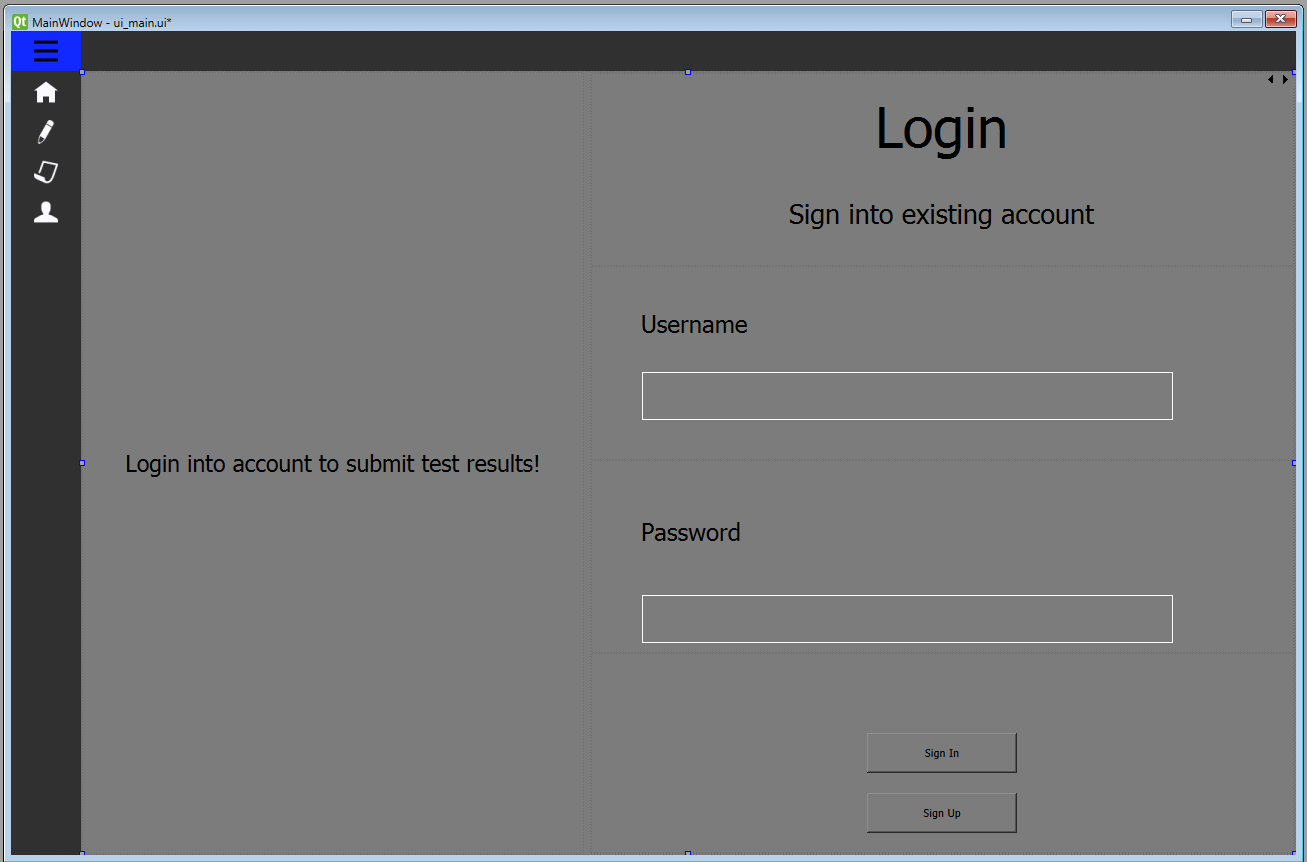
\includegraphics[width=0.9\textwidth]{GUI_designer}
  \caption{GUI design in Qt Designer}
  \label{Fig_SystemContext} 
  \end{center}
  \end{figure}

\wss{Include additional information related to the appearance of, and
interaction with, the user interface}

\section{Mechanical Hardware}

\section{Electrical Components}

\section{Communication Protocols}

\section{Reflection}

The information in this section will be used to evaluate the team members on the
graduate attribute of Problem Analysis and Design.  Please answer the following questions:

\begin{enumerate}
  \item What are the limitations of your solution?  Put another way, given
  unlimited resources, what could you do to make the project better? (LO\_ProbSolutions)
  \item Give a brief overview of other design solutions you considered.  What
  are the benefits and tradeoffs of those other designs compared with the chosen
  design?  From all the potential options, why did you select documented design?
  (LO\_Explores)
\end{enumerate}

\end{document}